\section{Neural Network}
\begin{definition}
A $d$-layer neural network (NN) is defined as the composition of the following components:
	\begin{itemize}
		\item Linear functions $L(\bfx) = \bfW \bfx + b: \R^{n} \rightarrow \R^{m}$, $\bfW \in \R^{n \times m}, b \in \R$;
		\item Activation function $\alpha(\bfx): \R^{m} \rightarrow \R^{m}$.
	\end{itemize}
	alternatively applied to the input data $\bfx \in \cX$, i.e.,
	$$
	NN(\bfx) = \alpha^{(d)} \circ L^{(d)} \circ \cdots \circ \alpha^{(1)} \circ L^{(1)}(\bfx).
	$$
	Here, $\circ$ is the composition operator.
\end{definition}

\begin{figure}[h]
\center
	\tikzset{%
  every neuron/.style={
    circle,
    draw,
    minimum size=0.8cm,
    line width=1pt,
    fill=gray!10
  },
  neuron missing/.style={
    draw=none, 
    scale=1,
    text height=0.333cm,
    fill=white,
    execute at begin node=\color{black}$\vdots$
  },
}

\begin{tikzpicture}[x=1.5cm, y=1cm, >=stealth]

\foreach \m/\l [count=\y] in {1,2,3,missing,4}
  \node [every neuron/.try, neuron \m/.try] (input-\m) at (0,2.5-\y) {};

\foreach \m [count=\y] in {1,missing,2}
  \node [every neuron/.try, neuron \m/.try ] (hidden-\m) at (2,2-\y*1.25) {};

\foreach \m [count=\y] in {1,missing,2}
  \node [every neuron/.try, neuron \m/.try ] (output-\m) at (4,1.5-\y) {};

\foreach \l [count=\i] in {1,2,3,n}
  \draw [<-] (input-\i) -- ++(-1,0)
    node [above, midway] {\small $x_\l$};

\foreach \l [count=\i] in {1,n}
  \node [above] at (hidden-\i.north) {\small $h^{(1)}_\l$};

\foreach \l [count=\i] in {1,n}
  \draw [-{>[scale=2.5,length=2,width=6]}] (output-\i) -- ++(1,0)
    node [above, midway] {\small $h^{(2)}_\l$};

\foreach \i in {1,...,4}
  \foreach \j in {1,...,2}
    \draw [-{>[scale=2.5,length=2,width=6]}] (input-\i) -- (hidden-\j);

\foreach \i in {1,...,2}
  \foreach \j in {1,...,2}
    \draw [-{>[scale=2.5,length=2,width=6]}] (hidden-\i) -- (output-\j);

\foreach \l [count=\x from 0] in {\small ${h}^{(0)} = \bfx$, \small ${h}^{(1)} = \alpha^{(1)} \circ L^{(1)}$, \small ${h}^{(2)} = \alpha^{(2)} \circ L^{(2)}$}
  \node [align=center, above] at (\x*2,2) {\l};
\end{tikzpicture}
\vspace{2mm}
\caption{Illustration of a 2-layer neural network}
\label{fig:MLP}
\end{figure}

\subsection{Gradients in NN}
(Omitted here. Please see the Ex. 6 for details.)

\section{Variational Autoencoder}

\subsection{InfoMax Principle}
Let $X$ and $Z$ be a measurement and a representation space, respectively. Let $F = \{\mathrm{enc}_\theta: \theta \in \Theta\}$ be a parametric family of function with $\mathrm{enc}_\theta: X \rightarrow Z$.

\begin{definition}[Mutual Information]
	The mutual information between $X$ and $Z$ is
	$$
	I(X; Z) = \EE_{X,Z}\left[ \log \frac{p(X, Z)}{p(X)p(Z)} \right]
	$$
\end{definition}

\begin{definition}[InfoMax Principle]
	Given a training set $\{x_1, \cdots, x_n\} \in X$, we can do the following approximation 
	$$
	\begin{aligned}
			\argmax_\theta\ I(X; Z) &= \argmax_\theta\ \EE_{X,Z}\left[ \log \frac{p(X, Z)}{p(X)p(Z)} \right] \\
			&= \argmax_\theta\ \EE_{X, Z}\left[ \log p(X \mid Z) \right] - \EE_{X}\left[ \log p(X) \right] \\
			&= \argmax_\theta\ \EE_X \EE_{Z \mid X} \left[ \log p(X_i \mid Z) \right] \\
			&\approx \argmax_\theta\ \sum_{i \leq n} \EE_{Z \mid X} \left[ \log p(X_i \mid Z) \right] 
	\end{aligned}
	$$
	
\end{definition}

\subsection{Variational Autoencoder}

\begin{align}
	& \argmax_{\theta, \theta', \phi}\  \sum_{i \leq n} \log p_{\theta', \theta}(x_i) \\
	=& \argmax_{\theta, \theta', \phi}\  \EE_{Z \sim q_\phi(\cdot \mid x_i)}[\log p_{\theta', \theta}(x_i)] \\
	=& \argmax_{\theta, \theta', \phi}\ \EE_{Z \sim q_\phi(\cdot \mid x_i)}\left[ \log \left(\frac{p_{\theta', \theta}(x_i, Z)}{p_{\theta', \theta}(x_i \mid Z)} \frac{q_\phi(Z \mid x_i)}{q_\phi (Z \mid x_i)} \right) \right] \\
	=& \argmax_{\theta, \theta', \phi}\ \underbrace{\EE_{Z \sim q_\phi(\cdot \mid x_i)}\left[ \log \left(\frac{p_{\theta', \theta}(x_i, Z)}{q_\phi(Z \mid x_i)} \right) \right]}_{\mathrm{ELBO\ of\ } \theta', \theta, \phi } + \underbrace{\EE_{Z \sim q_\phi(\cdot \mid x_i)}\left[ \log \left(\frac{q_\phi(Z \mid x_i)}{p_{\theta', \theta}(Z \mid x_i)} \right) \right]}_{KL\left[ q_\phi( \cdot \mid x_i) \ ||\   p_{\theta, \theta'}(\cdot \mid x_i)\right] \,\geq\, 0}
\end{align}
Note that $p_{\theta', \theta}(x_i, Z) = p_\theta(x_i \mid Z) \, p_{\theta'}(Z)  $. we have 
\begin{equation}
	\mathrm{ELBO} = \underbrace{\EE_{Z \sim q_\phi(\cdot \mid x_i)} [\log p_\theta(x_i \mid Z)]}_{\mathrm{Mutual\ Information:\ } I(X; Z)} + \underbrace{\EE_{Z \sim q_\phi(\cdot \mid x_i)} \left[ \log\left( \frac{p_{\theta'}(Z)}{q_\phi (Z \mid x_i)} \right) \right]}_{-KL\left[ q_\phi( \cdot \mid x_i) \ ||\  p_{\theta'}\right] }
\end{equation}
\remark The Mutual Information term encourage the representation to be infomrative, and KL divergence term tries to disentangle the encoder and decoder. 
\begin{figure}[htbp]
	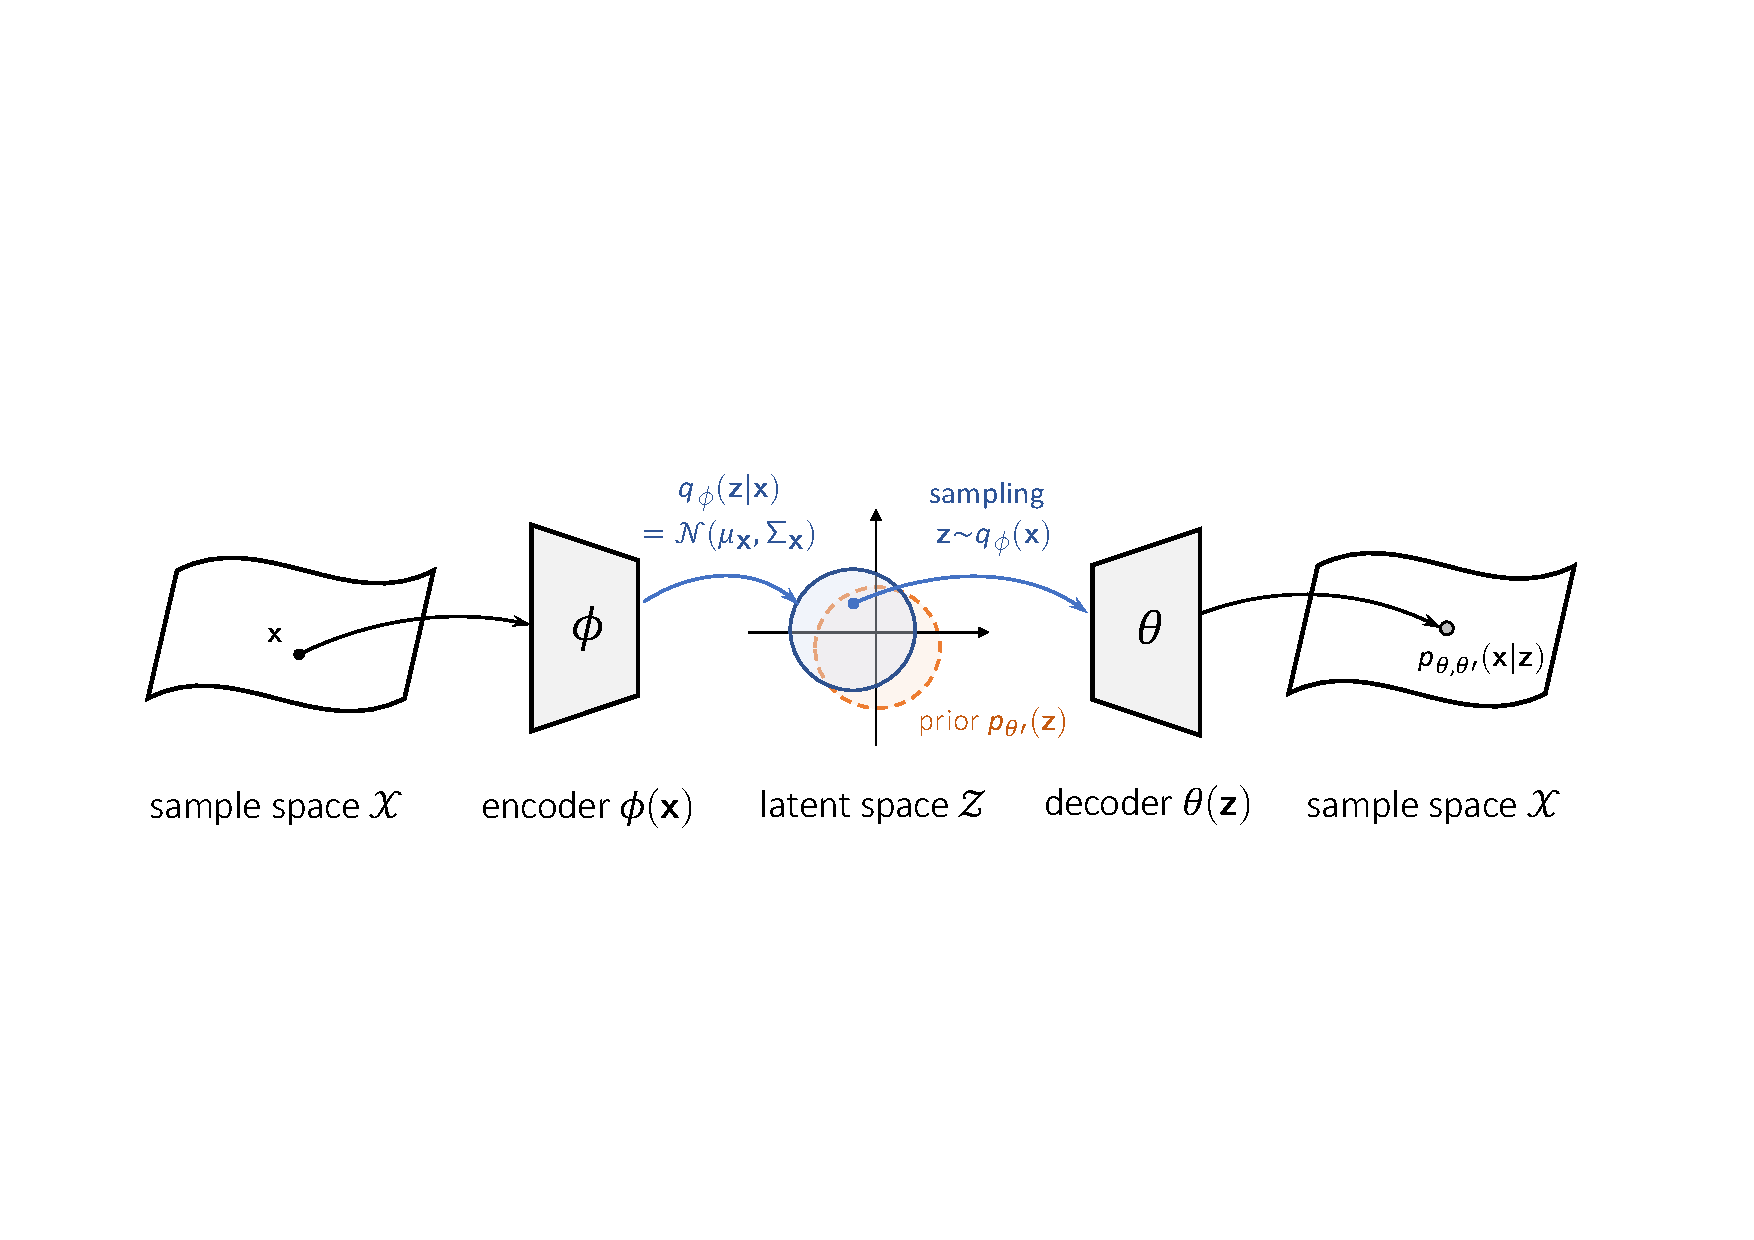
\includegraphics[width=\linewidth]{figures/vae}
	\caption{Illustration for Variational Autoencoder}
\end{figure}

\section{Optimization Methods}
\subsection{Newton's Method}
Newton’s method was originally created to find a root $f(\bfx^*) = 0$ of a given function $f(\bfx)$ via the iteration.
\begin{definition}[Newton's Method] Given a function $f: \cX \rightarrow \R$ and a initial value of $\bfx_0 \in \cX$, Newton’s method finds a root of $f(\bfx^*) = 0$ near $\bfx_0$ by iteration steps as
$$
	\bfx_{n+1} = \bfx_n - \frac{f(\bfx_n)}{f'(\bfx_n)},
$$
where $f'(\bfx)$ denotes the derivative of $f$ with respect to $\bfx$.
\end{definition}
In optimization we are usually interested in finding the minimum of a function. This can be achieved using Newton’s method to find a root of the first derivative $f'(\bfx^*) = 0$, the optimization step then becomes
\begin{equation}
	\bfx_{n+1} = \bfx_n - \frac{f'(\bfx_n)}{f''(\bfx_n)}.
\end{equation}
When applying in the high-dimensions, we have the form as
	\begin{align}
		\bfx_{n + 1} = \bfx_{n} -\mathbf{H}_f^{-1}(\bfx_{n}) \nabla_f(\bfx_{n})
	\end{align}

\begin{property}[Convergence of Newton's Method] \marginpar{\footnotesize A sequence $x_n$ converges with order $m$ towards $x^*$, if there exists a
constant $C$, such that $|x_n-x^*| \leq C |x_n-x^*|^m$} We call a smooth function $f$ with one root $f(x^*) = 0$ has order $k$, if its all derivatives $f^{(i)}(x^*) = 0,$ $\forall i > k$ and $f^{(k)}(x^*) \neq 0$.
	 Newton’s method converges linearly $(m = 1)$ for the function $f$ of order $k > 1$ in a region around the point $x^*$.
\end{property}

\begin{property}[Limits of Newton's Method] Newton's Method does not always work.  For example, it will never converge for $f(x) = \sqrt[3]{x}$ with $x_0 \neq 0$.
\end{property}
\begin{proof}
	Simply, we have
	\begin{equation}
		x_{n+1} = x_n - \frac{f(x_n)}{f'(x_n)} = x_n - \frac{x_n^{1/3}}{x_n^{-2/3} / 3} = -2x_n
	\end{equation}
	It will not converge, since $\lim_{n\rightarrow \infty} |x_n| = \infty, \forall x_0 \neq 0$.
\end{proof}

\subsection{Gradient Descent}
\begin{definition}
In gradient descent (GD), we iteratively estimate $\min_\bfw f(\bfw)$ by computing a sequence of estimates $\bfw^{(0)}, \cdots, \bfw^{(k)}, \cdots$. Each estimate $\bfw^{(k+1)}$ is obtained from the previous by adding an update in the direction against gradients $-\nabla_f(\bfw^{(k)})$ with step length of $\eta_k$, i.e.,
\begin{equation}
	\bfw^{(k+1)} \leftarrow \bfw^{(k)} - \eta_k \nabla_f(\bfw^{(k)}).
\end{equation}
\end{definition}
\begin{property}[Optimal Update of GD]
	Assume that $f$’s Hessian is invertible when evaluated at any point, then the optimal update is \marginpar{\footnotesize This is very similar to Newton's Method.}
	$$
	\Delta_k = -\mathbf{H}_f^{-1}(\bfw^{(k)}) \nabla_f(\bfw^{(k)}), 
	$$
	where $\mathbf{H}_f$ is the Hessian matrix of $f$.
\end{property}
\begin{proof}
	Let the optimal update of $k + 1$ step is $\bfw^{(k+1)} = \argmin_{\bfw} f(\bfw)$, where $\bfw \in U(\bfw^{(k)})$. Using Taylor's expansion of $f$ at $\bfw^{(k)}$, we have
	\begin{align}
		f(\bfw^{(k+1)}) = & \ f(\bfw^{(k)}) + (\bfw^{(k+1)} - \bfw^{(k)}) \nabla_f(\bfw^{(k)}) \\ & + \onehalf (\bfw^{(k+1)} - \bfw^{(k)})^\top \mathbf{H}_f(\bfw^{(k)}) (\bfw^{(k+1)} - \bfw^{(k)}) + o.
	\end{align}
	Set $ \diff{\bfw}f(\bfw) = 0$, we get
	\begin{align}
		\bfw^{(k + 1)} = \bfw^{(k)} -\mathbf{H}_f^{-1}(\bfw^{(k)}) \nabla_f(\bfw^{(k)})
	\end{align}
\end{proof}

\noindent \remark When applying optimal update, GD is equivalent to Newton's method. The drawback is that Newton's method relies on the inverse of Hessian matrix, which may be intractable in practical.

\begin{property}[Optimal Learning Rate]
	The optimal learning rate $\eta_k$ is the learning rate such that $\bfw^{(k)} - \eta_k \nabla_f(\bfw^{(k)})$ takes the minimal value.
\end{property}
\begin{proof}
	Similar to the previous one, we have the Taylor's expansion of $f$ at $\bfw^{(k)}$ as
	\begin{align}
		f(\bfw^{(k+1)}) \approx & \ f(\bfw^{(k)}) + (\bfw^{(k+1)} - \bfw^{(k)}) \nabla_f(\bfw^{(k)}) \\ & + \onehalf (\bfw^{(k+1)} - \bfw^{(k)})^\top \mathbf{H}_f(\bfw^{(k)}) (\bfw^{(k+1)} - \bfw^{(k)}) \\
		= &  \ f(\bfw^{(k)}) - \eta_k \nabla_f(\bfw^{(k)})^\top \nabla_f(\bfw^{(k)}) + \onehalf \eta_k^2 \nabla_f(\bfw^{(k)})^\top \mathbf{H}_f(\bfw^{(k)}) \nabla_f(\bfw^{(k)})
	\end{align}
	Set $ \diff{\eta_k}f(\bfw) = 0$, we get
	\begin{equation}
		0 = \diff{\eta_k}f(\bfw) = - \norm{ \nabla_f(\bfw^{(k)}) }^2 + \eta_k \nabla_f(\bfw^{(k)})^\top \mathbf{H}_f(\bfw^{(k)}) \nabla_f(\bfw^{(k)})
	\end{equation}
	Therefore, the optimal learning rate is
	\begin{equation}
		\eta_k = \frac{\norm{ \nabla_f(\bfw^{(k)}) }^2}{\nabla_f(\bfw^{(k)})^\top \mathbf{H}_f(\bfw^{(k)}) \nabla_f(\bfw^{(k)})}.
	\end{equation}
\end{proof}

\subsection{Robbins-Monro Algorithm}
\begin{definition}
	Given a function $f: \R^m \times \R^n \rightarrow \R$ and a random variables $Z \in \R^m$ whose distribution is unknown. The goal is to compute $\theta^*$ such that $\E{\bfz\sim Z}{f(\bfz; \theta)} = 0$ via iteration as
\begin{equation}
	\theta^{(k + 1)} = \theta^{(k)} - \eta^{(k + 1)}f(\bfz_{k + 1}; \theta^{(k)}),
\end{equation}
where $\eta^{(k)}$ denotes the learning rate at each step, and samples $ \bfz_1, \cdots, \bfz_k \sim Z$.
\end{definition}
\begin{theorem}[Convergence]
If $\E{\bfz \sim Z}{f(\bfz; \theta)} $ satisfies following regularity conditions
$$
\eta^{(k)} \geq 0, \quad \sum_k \eta^{(k)} = \infty, \quad \sum_k \eta^{(k) 2} < \infty,
$$
then Robbins-Monro algorithm will converge to $\theta^*$ with probability $1$.
\end{theorem}
\begin{proof}
	The proof can be found in Ex.4 - 4, or at \footnote{K. Fukunaga. Introduction to Statistical Pattern Recognition.}.
\end{proof}

\begin{definition}[Regularity Conditions]
	If certain sufficient conditions are meet, then Robbins-Monro algorithm will converge to $\theta^*$. These conditions are called regularity conditions, which are
\begin{align*}
	\E{Z}{f(Z; \theta^*)} & < \E{Z}{f(Z; \theta)}, \forall \theta > \theta^*, \\
	\E{Z}{f(Z; \theta^*)} & > \E{Z}{f(Z; \theta)}, \forall \theta < \theta^*. 
\end{align*}
\end{definition}

\subsection{Stochastic Gradient Descent}
Stochastic Gradient Descent (SGD) is an example of Robbins-Monro algorithm. 
\begin{definition}
	\begin{equation}
		\min_\theta \sum_{i \leq n} \cL(y_i, NN_\theta(\bfx_i))
	\end{equation}
\end{definition}
\begin{tabular}{p{5.5cm} p{4cm} p{4cm}}
\toprule
	& \textbf{Batch GD} & \textbf{Mini-batch GD} \\
	\midrule
Gradient precision & High & Low \\
Handling large training set & Bad & Good \\
Improvement & Slow & Fast \\
Escaping local minimal & Not likely & Likely \\
Generalization error & High & Low \\
\bottomrule
\end{tabular}